\documentclass[a4paper,12pt]{scrartcl} 

%% \usepackage[latin1]{inputenc}
%%apt-get install texlive-lang-german kile kile-l10n  aspell-de  texlive-fonts-extra
%%damit ngerman keine Probleme mehr macht !!
\usepackage[utf8]{inputenc} 
\usepackage[T1]{fontenc}
\usepackage[ngerman]{babel}

\usepackage{setspace}

\setcounter{tocdepth}{3}				%Schatelungstiefe Inhaltsverz.
\usepackage[utf8]{inputenc}			%deutsche Umlaute
\usepackage{german, ngerman}
\usepackage[ngerman]{babel}			%Rechtschreibprüfung
\usepackage{color,listings} 			%Quellcode Highlighting, bindet das
\usepackage{float}					%% GRAFIKPOSITION MITTELS [H] ERWZINGEN
%Paket Listings ein
\usepackage{listings}
\usepackage{color}
\usepackage{textcomp}
\usepackage[T1]{fontenc}				%srccode
\usepackage[scaled]{beramono}		%srccode
\usepackage{longtable}				%mehrseitige tabellen
\usepackage[tableposition=b]{caption}
\usepackage[pdftex, pdftoolbar=false, hyperfootnotes=false, bookmarks,
bookmarksopen, bookmarksnumbered, bookmarksopenlevel=2, pdfpagelabels=true,
pdfstartpage=3, pdfstartview=FitH,]{hyperref} %Verlinkungen
\usepackage{array}					%farbige Tabellen
\usepackage[table]{xcolor} 			%farbige Tabellen
\usepackage{graphicx}				% \includegraphics bnoetigt dies

\usepackage{fancyhdr, graphicx}		%% Logo auf Titelseite
\renewcommand{\headrulewidth}{0pt}
\fancyhead[L]{}
\fancyhead[R]{
  \includegraphics[width=52mm]{./images/htwk.png}
}

%%%% mathemathische Formeln zentrieren und vom Text absetzen mittels \[ E = mc^2 \] anstatt $ E = mc^2 $ %%%%
\usepackage{amsmath}
\usepackage{amsthm}
\usepackage{amsbsy}
\usepackage{amssymb}
%%%%%%%%%%%%%%%%%%%%%%%%%%%%%%%%%%%%%%%%%%%%%%%%%%%%%%%%%%%%%%%

\definecolor{Navy}{rgb}{0,0,0.5}
\definecolor{Gray}{gray}{0.5}
\definecolor{dunkelgrau}{rgb}{0.8,0.8,0.8}
\definecolor{hellgrau}{rgb}{0.95,0.95,0.95}
\definecolor{hellgrau2}{rgb}{0.93,0.93,0.93}

\hypersetup{
	colorlinks=true, 			% false: boxed links; true: colored links
	linkcolor=Navy,          		% color of internal links
	citecolor=Gray,        			% color of links to bibliography
	filecolor=magenta,      		% color of file links
	urlcolor=blue,           			% color of external links
	linkbordercolor={1 1 1}, 		% set to white
	citebordercolor={1 1 1} 		% set to white
}


%Einrückung eines neuen Absatzes
\setlength{\parindent}{0em}

%Definition der Ränder
\usepackage[paper=a4paper,left=30mm,right=30mm,top=30mm,bottom=30mm]{geometry}

%Abstand der Fussnoten
\deffootnote{1em}{1em}{\textsuperscript{\thefootnotemark\ }}

%Regeln, bis zu welcher Tiefe (section,subsection,subsubsection) Überschriften angezeigt werden sollen (Anzeige der Überschriften im Verzeichnis / Anzeige der Nummerierung)
%\setcounter{tocdepth}{3}
%\setcounter{secnumdepth}{3}

\fancypagestyle{htwkheader}
{
   \fancyhf{}	% clear all header and footer fields
  \fancyhead[RO]{
	\makebox[\textwidth]{	%% schiebe Logo nach aussen auf den Rand
		\rule{1				%% nach aussen schieben hoeherer Wert -> Logo weiter nach aussen
		  \textwidth}{0cm} %% nicht nach unten schieben = 0cm
			\includegraphics*[width=52mm]{./images/htwk.png}	%%Logo HTWK
	  }
  }
}



\begin{document}
 
%Beginn der Titelseite
\begin{titlepage}
\begin{small}
\vfill {HTWK Leipzig\\
Fachbereich IMN \\
Sommersemester 2014}
\end{small}
 
\begin{center}
\begin{Large}
\vfill {\textsf{\textbf{
Traincard\\
}}}
\end{Large}
Beleg im Smartcard Programmierung\\bei Prof. Dr. rer. nat. Uwe Petermann
\end{center}
 
\begin{small}

\vfill
Kurt Junghanns, B.Sc.\\
Marcel Kirbst, B.Sc. \\
Michael Reher, B.Sc.\\
\\
\today
\end{small}
 
\end{titlepage}
%Ende der Titelseite
 
%Inhaltsverzeichnis (aktualisiert sich erst nach dem zweiten Setzen)
\tableofcontents
%Abbildungsverzeichnis und Tabellenverzeichnis auf einer Seite
\clearpage
\listoffigures
\listoftables
\thispagestyle{empty}
 
\clearpage
\onehalfspacing
 
\pagestyle{plain}
 
\section{Einleitung}
\label{sec:0}
Diese Arbeit befasst sich mit der Vorstellung der Belegarbeit im Fach Smartcard Programmierung mit dem Thema ``Traincard''. 
Ziel des Belegs ist die prototypische Implementierung eines Trainingssystems auf Basis JCOP-fähiger Smartcards. 
\\
\\
Im ersten Kapitel \nameref{sec:1} wird der Use-Case für die prototypische Implementierung beschrieben, sowohl unter \nameref{subsec:1.1} aus Sicht des Trainierenden, wie auch unter \nameref{subsec:1.2} aus Sicht des Trainers.
%In Kapitel \nameref{sec:2} wird die Protokollfamilie IPv6 vorgestellt. Welche Probleme gelöst werden, wenn anstelle von IPv4, IPv6 verwendet wird, wird im Kapitel \nameref{sec:3} erläutert. Im Kapitel \nameref{sec:4} wird anhand eines Praxisbeispiels erläutert wie sich IPv6-Konnektivität an einem Rechnersystem kofigurieren lässt. Abschließend erfolgt im Kapitel \nameref{sec:5} eine Zusammenfassung der Arbeit.


%%Auch wenn klar sein muss, dass es im Umfang eines solchen Beleges nicht ann\"ahrend abschlie{\ss}end m\"oglich ist das Thema IPv6 ersch\"opfend vorzustellen, so hofft der Autor dem geneigten Leser doch einen \"Uberblick \"uber die Funktionen und Vorteile von IPv6 bieten zu k\"onnen.

\clearpage
\section{Anwendungsfall}
\label{sec:1}
In vielen Fitnessstudios werden heute noch bei der Neuanmeldung Trainingspläne auf Papier ausgegeben. Der Trainierende führt den Trainingsplan über die Trainingsperiode ständig bei sich und verzeichnet den Trainingsfortschritt in diesem Dokument.
Im Verlauf der Trainingsperiode kann der Trainer beurteilen wie effektiv das Training beim Trainierenden ist.\\
\\
Die Verwendung altmodischer Trainingspläne auf Papier hat jedoch einige Nachteile. Beispielsweise wird das Dokument vom Trainierenden manchmal vergessen, die betreffenden Trainingsfortschritte müssen also nachgetragen werden. 
Weiterhin sind Traingspläne in Papierform nicht besondern resistent gegen Abnutzung und verschleißen mit fortdauernder Verwendung. Um den genannten Nachteilen zu begegnen soll im Rahmen dieser Belegarbeit der Einsatz von Trainingsplänen
auf Basis so genannter Smartcards abgebildet werden. Smartcards können sehr leicht in einer Brieftasche mitgeführt werden und sind weniger anfällig für Abnutzung. Weiterhin bieten sich viele weitere Vorteile wie ... (Datenlogging für das Studio, Kopieren bzw. 
verteilter Zugriff auf die Daten ....) 


\subsection{Anwendungsfall aus Sicht des Trainierenden}
\label{subsec:1.1}

Aus Sicht des Trainierenden bietet die Verwendung der Smartcard einige der folgenden Vorteile:
\begin{itemize}
\item leichte Transportierbarkeit
\item robuster als Trainingspläne aus Papier
\end{itemize}


\subsection{Anwendungsfall aus Sicht des Trainers}
\label{subsec:1.2}
Trainer profitieren beim Einsatz von Smartcards unter anderem von folgenden Vorteilen:
\begin{itemize}
\item leichte und lesbare Auswertung der vorgegebenen Trainingspläne
\item zusätzliche Metainformationen wie beispielsweise zu welchem Zeitpunkt welcher Datensatz geschrieben wurde
\item statistische Auswertungen lassen sich sehr leicht erstellen 
\end{itemize}

\clearpage
\section{Grundlagen}
\label{sec:2}
In diesem Kapitel wird auf die Grundlagen der in diesem Beleg verwendeten Technologien eingegangen.

\subsection{Grundlagen Smartcard}
\label{subsec:2.1}
Die in diesem Beleg verwendete Smartcard basiert auf der Java Card Technologie. Die Java Card Technologie bietet eine 
Teilmenge der Java Programmiersprache, sowie eine hinsichtlich der Anforderungen an Smartcards optimierte Laufzeitumgebung.

Die Verwendung von Java-basierten Smartcards bietet einige Vorteile, von denen nachfolgend eine Auswahl beispielhaft genannt sei: \cite{jcopdoc}

\begin{description}
\item[plattformunabhängig:] Java Card Applets, die der Java Card API entsprechen, lassen sich plattformunabhängig und herstellerübergreifend nutzen.
\item[Multiapplikationsfähig:] es können mehrere Applikationen gleichzeitig auf einer Smartcard ausgeführt werden
\item[hohe Flexibilität:] die Verwendung der objektorientierten Programmiersprache Java erlaubt die Erstellung komplexer Anwendungen für die Smartcard.  
\item[Post-Aktualisierbarkeit:] die Möglichkeit, nachträglich Code auf der Smartcard zu modifizieren und auszutauschen erhöht die Flexibilität weiter
\item[Standardkonformität:] die Java Smartcards entsprechen dem ISO7816 Standard \cite{iso7816}
\end{description}

Eine Java Smartcard besteht im Wesentlichen aus den Bestandteilen Kommunikationsschnittstelle, Speicher und einem Prozessor zur Durchführung von Berechnungen.
Bei Verwendung der Smartcard wird diese in ein Lesegerät eingelegt. Das Lesegerät wird in einschlägiger Literatur auch als Card Acceptance Device, abgekürzt CAD, bezeichnet.
Der Speicher auf Java Smartcards besteht aus zwei Typen, RAM und EEPROM. Der RAM-Speicher ist flüchtig und kann beliebig oft beschrieben werden. Der EEPROM-Speicher ist nichtflüchtig und kann nur endlich oft beschrieben werden, je nach Hersteller und Modell bis zu 100.000 mal pro Speicherzelle.  

\subsection{JCOP}
\label{subsec:2.2}
Java von Neunzehnhundertzwieback \& co.

\subsection{APDU}
\label{subsec:2.3}

Die Kommunikation zwischen dem Kartenlesegerät und der Smartcard erfolgt reaktiv und paketweise. Reaktiv bedeutet, dass die Smartcard keine Kommunikation initiiert sondern nur auf Anfragen vom Lesegerät reagiert. Der bei der Kommunikation zwischen Smartcard und Lesegerät verwendete Kommunikationsmechanismus wird als Application Protocol Data Units, abgekürzt APDU, bezeichnet. Spezifiziert ist dies ebenfalls in ISO7816 Teil 4.\cite{iso7816}
\\

\begin{figure}[htb]
\begin{center}
 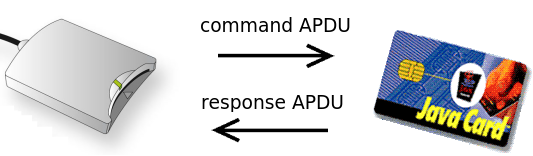
\includegraphics[width=1\hsize]{./images/apdu.png}
\end{center}
\caption[APDU-Kommunikation schematisch dargestellt, Quelle: Autoren]{\label{apdu}APDU-Kommunikation schematisch dargestellt, Quelle: Autoren}
\end{figure}

Die Kommunikation wird über ein so genanntes command APDU Paket initiiert, welches aus den folgenden Feldern besteht:


\begin{description}
\item[CLA:] class,gibt die Klasse an, spezifiziert ob es sich um ein ISO7816-4 konformes Kommando handelt
\item[INS:] gibt die Instruktion an
\item[P1:] zusätzlicher Parameter
\item[P2:] zusätzlicher Parameter
\end{description} 

Weiterhin können je nach Kommandotyp noch die folgenden, optionalen Felder an das command APDU Paket angehängt werden:


\begin{description}
\item[Lc:] Length, gibt die Länge der Kommandodaten
\item[Data:] gibt die Kommandodaten an
\item[Le:] gibt die Länge der erwarteten Antwort an
\end{description}

Als Antwort erhält das Lesegerät von der Smartcard ein so genanntes response APDU Paket. Dieses Antwortpaket kann Daten enthalten, dies ist jedoch nicht obligatorisch. 


\clearpage
\section{Umsetzung}
\label{sec:3}

Dieses Kapitel legt die Umsetzung dar.

\subsection{Systemumgebung}
\label{subsec:3.1}

%Aufteiung in off- und oncard
%oncard ist applet auf emulierter smartcard, welche in der JCOP Eclipse Umgebung ausgeführt wird
%Die Smartcard wird per $/close$ Befehl von der JCOP debug Konsole gelöst und ist über den Port 8090 erreichbar
%der offcard teil ist ebenfalls in Java programmiert
%sofern entsprechende firewall regeln erstellt wurden sind, kann sich der on -und offcard teil auf verschiedenen rechnern befinden
%Der oncard muss ebenso wie der offcard teil einzeln gestartet werden, wonach beide Teile direkt miteinander kommunizieren
%Der Inhalt der APDUs orientiert sich stark an der ISO Norm ISO7816. Der konkrete Aufbau ist in Abbildung apdu.png zusehen (NOA=Number of APDUs)

%Die Modelklassen besitzen Funktionen zur umwandlung zwischen instanzen und byte Arrays zur Übertragung
%diese umwandlung  wurde eigens implementiert und orientiert sich am Aufbau von ethernet Packeten. Ein Packet besteht dabei immer aus einem byte für einen eindeutigen Identifikator, zwei bytes für die anzahl der data bytes sowie bytes für den dateninhalt

Da für die Umsetzung des Belegs keine Experimentalhardware zur Verfügung steht, erfolgt die Implementierung mit Hilfe eines Simulators.

\subsection{On-Card Teil}
\label{subsec:3.2}
Der On-Card Teil der Implementierung enthält sämtliche Trainingspläne und weitere Daten.

%Der Oncard Teil ist mit der Klasse Traincard im Packet htwk.smartcard.traincard abgebildet. +klassendiagramm

%das applet empfängt anfragen, wertet diese aus und sendet Daten oder ein erfolgsbyte im datenbereich zurück
%Daten werden dabei immer als byte arrays geschrieben und gelesen

\subsection{Off-Card Teil}
\label{subsec:3.3}

% der offcard Teil besteht aus der graphischen Oberfläche, der Logik zur Steuerung der Oberfäche und der Logik zur Kommunikation mit der Smartcard

\clearpage
\section{Zusammenfassung und Ausblick}
\label{sec:5}
Zusammenfassung und Ausblick ohne persönliche Meinung.

\clearpage
\section{Quellenverzeichnis}
\label{sec:6}
\renewcommand\refname{Quellenverzeichnis}
\begin{thebibliography}{999}

\bibitem{jcopdoc}Sun Microsystems, Inc.:  {\sl Java Card Applet Developer's Guide}\\
\url{http://www.oracle.com/technetwork/java/javacard/downloads/index.html}\\
abrufbar am 01.Juli 2014

\bibitem{iso7816}International Organization for Standardization: {\sl ISO 7816 - Identification cards -- Integrated circuit cards}
kostenpflichtig abrufbar unter \url{http://www.iso.org/}

\bibitem{label01}Autornachname, Autorvorname:  {\sl Buchtitel} Verlag, Erscheinungsjahr,
\\ISBN:  978-0-07024-807-6

\bibitem{dittler2002}Uwemann, Peter:  {\sl Train harder, 2. Auflage}. gpunkt-Verlag Heidelberg, 2012,
\\ISBN: 133-7-13371-337-1


\end{thebibliography}
\end{document}